\documentclass[12pt]{article}
\usepackage{fontspec}
\setmainfont{Times New Roman}
\usepackage[legalpaper,margin=0.8in]{geometry}
\usepackage{xcolor}
\usepackage{amsmath}
\usepackage{graphicx}
\usepackage{caption}
\usepackage{longtable} % For long tables spanning multiple pages
\usepackage{array}
\usepackage{makecell}
\usepackage{setspace}
\onehalfspacing % Για απόσταση 1.5 γραμμών

\title{Η απόδοση των μαθητών λαμβάνοντας υπόψη παράγοντες της καθημερινότητας τους}




\author{Ιωάννου Νικόλας - ge20718 
\\ Μπέκος Θοδωρής - ge}
\date{Δεκέμβριος 2024}


\begin{document}
\maketitle

\vspace{0.7cm}
\begin{center}
    
\includegraphics[width=0.7\textwidth]{./images/Εθνικό_Μετσόβειο_Πολυτεχνείο.svg}
    
    \Large Σχολή εφαρμοσμένων μαθηματικών και φυσικών επιστημών \\[1.5cm]
\end{center}



        
\vfill


        \noindent\Large Μάθημα: ΘΕΜΑ \\[0.5cm]


        \noindent\textbf{Υπέυθυνος καθηγητής:} 
        Δρ. Στεφανέας Πέτρος \\[1cm]

\newpage
\noindent\textbf{Ευχαριστίες:} \\

\noindent Θα θέλαμε να ευχαριστήσουμε τον κύριο Πέτρο Στεφανέα για το ενδιαφέρον και
την εμπιστοσύνη που μας έδειξε κατά τη διάρκεια πραγματοποίησης της εν λόγω εργασίας. Επίσης, θα θέλαμε να ευχαριστήσουμε τις οικογένειες μας γιατί χωρίς αυτές δεν θα μπορούσαμε να βρισκόμασταν στη θέση που βρισκόμαστε τώρα.

\newpage
\renewcommand{\contentsname}{\Huge \textbf{Περιεχόμενα}}

% Πίνακας περιεχομένων
\tableofcontents
\newpage

\section{Εισαγωγή}
km
\newpage

\section{Introduction}
gt
\newpage
\section{Ανάλυση της διαδικασίας επιλογής μοντέλου}
\subsection{Ανάλυση του προβλήματος}

Το πρόβλημα το οποίο αντιμετωπίσαμε έχει να κάνει με την κατασκευή μοντέλου μηχανικής μάθησης για την πρόβλεψη των βαθμών των μαθητών μέσω διαφόρων παραγόντων που θα αναλύσουμε παρακάτω. Το πρόβλημα αυτό αποτελεί πρόβλημα παλινδρόμισης αφού ο τελικός βαθμός δεν αποτελεί κατηγορική αλλά ποσοτική μεταβλητή και παίρνει συνεχείς τιμές. Χρησιμοποιήσαμε το σύνολο δεδομένων  Student Performance Factors που βρήκαμε στο Kaggle ,όπου τα χαρακτηριστικά τα οποία το αποτελούν φαίνονται στον πίνακα παρακάτω:\\

\begin{center}
\begin{longtable}{|p{5cm}|p{7.1cm}|p{4cm}|} % Creates a table with 3 columns, all centered, with borders
\hline
Χαρακτηριστικά & Περιγραφή & Εύρος τιμών \\ % Header row
\hline
Attendance & Ποσοστό μαθημάτων που παρευρέθηκε ο μαθητής & 0-100 \\ % Row 1
\hline
Previous Scores & Μέσος όρος βαθμών απο προηγούμενες εξετάσεις & 0-100 \\ % Row 7
\hline
Sleep Hours & Ώρες ύπνου ανά μέσο όρο κάθε βράδυ & 4-10 \\ % Row 6
\hline
Hours Studied & Αριθμός ωρών που δίαβασε ο μαθητής μέσα στην βδομάδα & 0-50 \\ % Row 2
\hline
Tutoring Sessions & Αριθμός φροντιστηριακών μαθημάτων ανά μήνα & 0-10 \\ % Row 10
\hline
Family income & Οικογενειακό εισόδημα & Low/Medium/ High \\ % Row 11
\hline
Teacher quality & \makecell[l]{Εκπαιδευτική ικανότητα\\ καθηγητή} & Low/Medium/ High \\ % Row 12
\hline
\makecell[l]{Parental\\ Involvement} & Βαθμός εμπλοκής γονέων στην εκπαίδευση του μαθητή & Low/Medium/ High \\ % Row 3
\hline
Access to Resources & Πρόσβαση μαθητή σε εκπαιδευτικό υλικό & Low/Medium/ High \\ % Row 4
\hline
Motivation Level & Κίνητρο μαθητή & Low/Medium/ High \\ % Row 8
\hline
Peer Influence & \makecell[l]{Επιρροή μαθητή απο\\ ομήλικους του} & \makecell[l]{Negative/\\ Neutral/ \\Positive} \\ % Row 14
\hline
Distance from home & Απόσταση σχολείου απο το σπίτι & Near/Moderate/ Far \\ % Row 18
\hline
School type & Τύπος σχολείου & Private/Public \\ % Row 13
\hline

Physical activity & \makecell[l]{Επίπεδο φυσικής \\ δραστηριότητας μαθητή} & \makecell[l]{Sedentary/ \\ Light/Moderate/ \\ Active/ \\ Very Active/ \\ Highly Active/ \\ Athlete} \\ % Row 15
\hline

Parental education level & Επίπεδο εκπαίδευσης γονέα & \makecell[l]{High School/ \\ College/ \\ Postgraduate} \\ % Row 17
\hline
Extracurricular activities & Εξωσχολικές δραστηριότητες & Yes/No \\ % Row 5
\hline
Learning disabilities & Μαθησιακές δυσκολίες & Yes/No \\ % Row 16
\hline

Internet Access & Πρόσβαση στο διαδίκτυο & Yes/No \\ % Row 9
\hline
Gender & Φύλο μαθητή & Male/Female \\ % Row 19
\hline

Exam Score & Βαθμός εξέτασης & 0-100 \\ % Row 20
\hline
\end{longtable}
\end{center}

Η μεταβλητή Exam Score αποτελεί την εξαρτημένη μεταβλητή(στόχο) του μοντέλου ενώ οι υπόλοιπες μεταβλητές αποτελούν τις πιθανές ανεξάρτητες μεταβλητές. 


\subsection{Επεξεργασία των δεδομένων}
Ρίχνωντας μια ματιά στα δεδομένα μπορούμε να παρατηρήσουμε πως υπάρχουν παρατηρήσεις με ελλειπείς τιμές. Σε αυτή την περίπτωση έχουμε 3 επιλογές. Η πρώτη επιλογή είναι να διαγράψουμε τις παρατηρήσεις αυτές, η δεύτερη να προβλέψουμε τις τιμές των παρατηρήσεων με κάποια μέθοδο (Παλινδρόμιση για τις ποσοτικές και ομαδοποίηση για της κατηγορικές μεταβλητές) και η τρίτη να αντικαταστήσουμε τις ελλειπείς τιμές με κάποιο λογικό τρόπο(π.χ. εάν έχουμε ποσοτικές τιμές με την μέση τιμή του χαρακτηρηστικού ή εάν έχουμε κατηγορική με την τιμή, η οποία εμφανίζεται τις περισσότερες φορές). Επιλέξαμε να διαγράψουμε τις παρατηρήσεις οι οποίες έχουν ελλειπείς τιμές μιας και ο αριθμός των παρατηρήσεων είναι ικανοποιητικός και οι ελλειπεις τιμές αποτελούν ένα πολύ μικρό ποσοστό(<10\(\%\)) των συνολικών παρατηρήσεων και δεν θα επιρεάσουν το αποτέλεσμα. 

Η μεταβλητή Physical Activity εχει μια ιδιαιτερότητα. Παρόλο που περιέχει αριθμητικές τιμές(0-6), αυτές οι τιμές αποτελούν κατηγορίες. Για αυτό και εμείς αλλάξαμε τον τύπο της μεταβλητής σε αντικείμενο. Μπορούμε να παρατηρήσουμε πως το dataset μας τώρα έχει 14 κατηγορικές μεταβλητές και 6 ποσοτικές.

Για να κατανοήσουμε καλύτερα τα δεδομένα μας θα χρησιμοποιήσουμε διάφορες αριθμητικές και γραφικές μεθόδους. Για της ποσοτικές μεταβλητές θα υπολογίσουμε την μέση τιμή, την διασπορά, το εύρος, το ενδοτεταρτημοριακό εύρος, την διάμεσο, το πρώτο τεταρτημόριο(Το 25\(\%\) των τιμών της μεταβλητής είναι μικρότερα απο αυτή την τιμή), το τρίτο τεταρτημόριο(Το 75\(\%\) των τιμών της μεταβλητής είναι μικρότερα απο αυτή την τιμή) και την μέγιστη και ελάχιστη τιμή τους. Επίσης, θα κατασκευάσουμε τον πίνακα Pearson των μεταβλητών όπως και τα ιστογράμματα και θηκογράμματα τους τα οποία παρουσιάζονται παρακάτω:

\begin{center}
    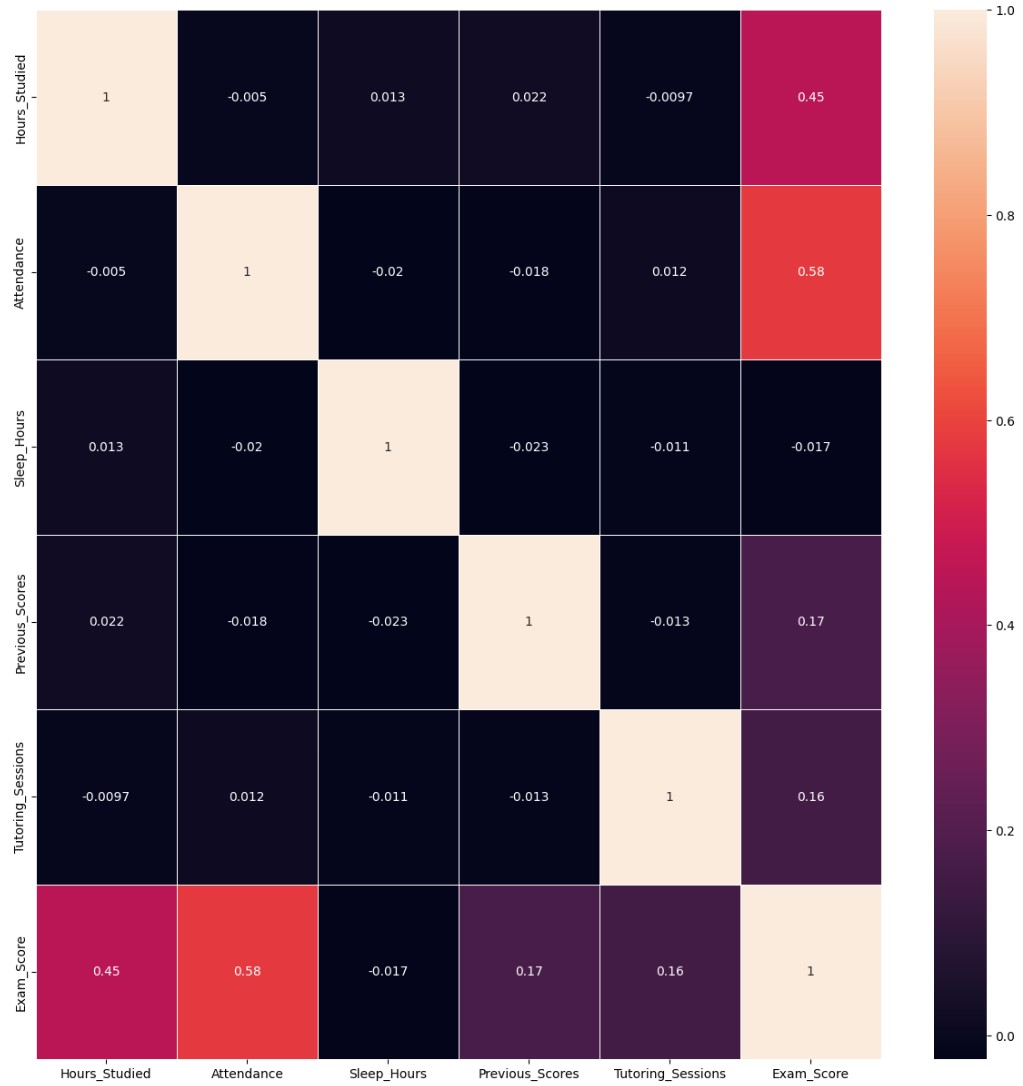
\includegraphics[width=1\textwidth]{./images/icon1.jpg}
    
\end{center}

Ο πίνακας Pearson δείχνει την γραμμική συσχέτιση μεταξύ των ποσοτικών μεταβλητών.

\begin{center}
    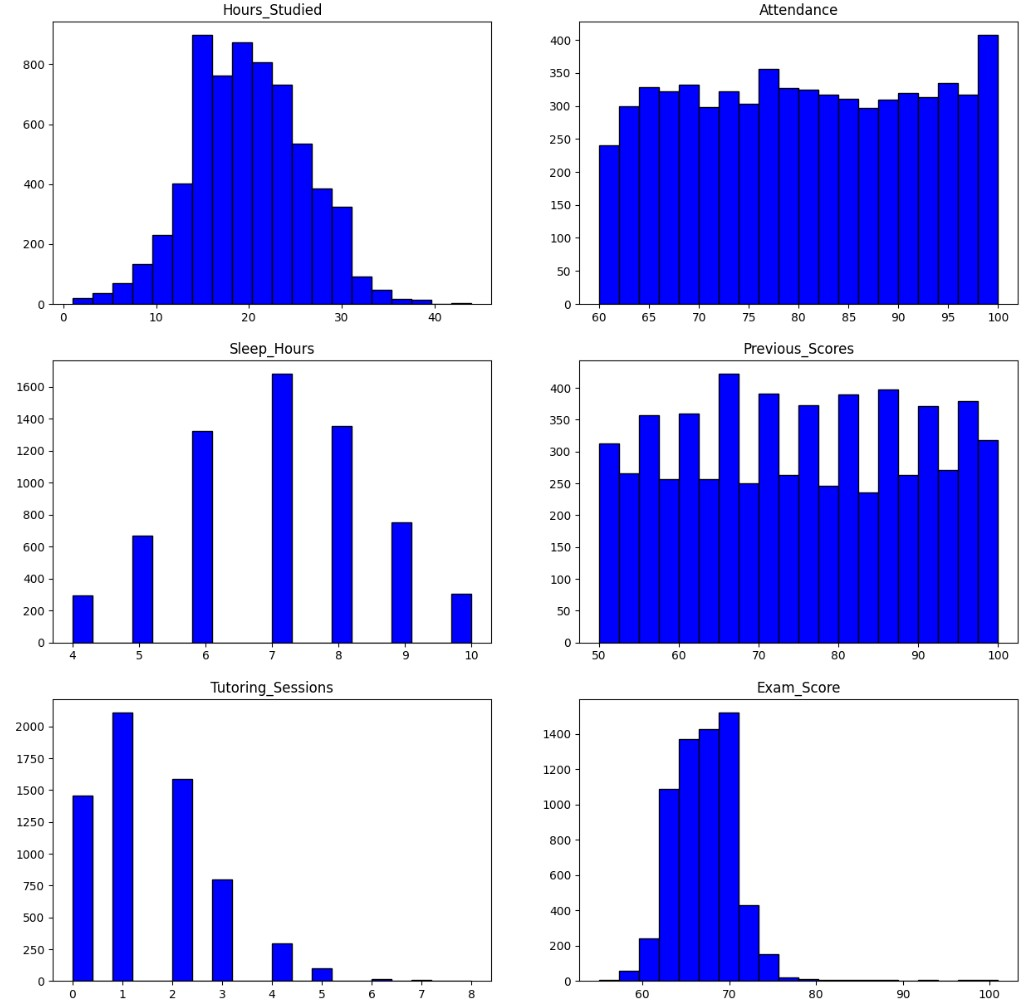
\includegraphics[width=1\textwidth]{./images/icon2.jpg}
    
   
\end{center}

\begin{center}
    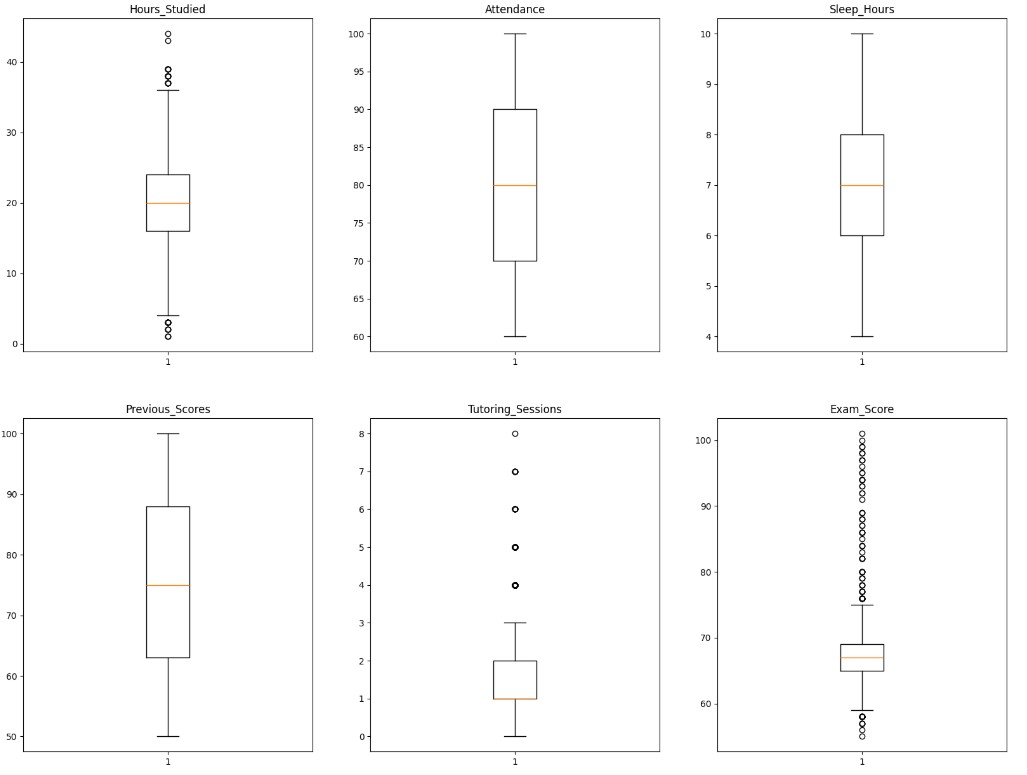
\includegraphics[width=1\textwidth]{./images/icon3.jpg}
    
\end{center}

Απο τα παραπάνω διαγράμματα μπορούμε να αντλήσουμε χρήσιμες πληροφορίες οι οποίες θα μας φανούν σημαντικές στην πορεία.

Αντίστοιχα για τις κατηγορικές μεταβλητές υπολογίζουμε τον αριθμό των κατηγοριών, την τιμή η οποία εμφανίζεται τις περισσότερες φορές όπως και το πλήθος της συγκεκριμένης τιμής στην μεταβλητή. Στη συνέχεια κατασκευάζουμε τον πίνακα Cramers' V , τα ραυδογράμματα των κατηγορικών μεταβλητών όπως και ο πίνακας ANOVA μεταξύ των ποσοτικών και κατηγορικών μεταβλητών.

\begin{center}
    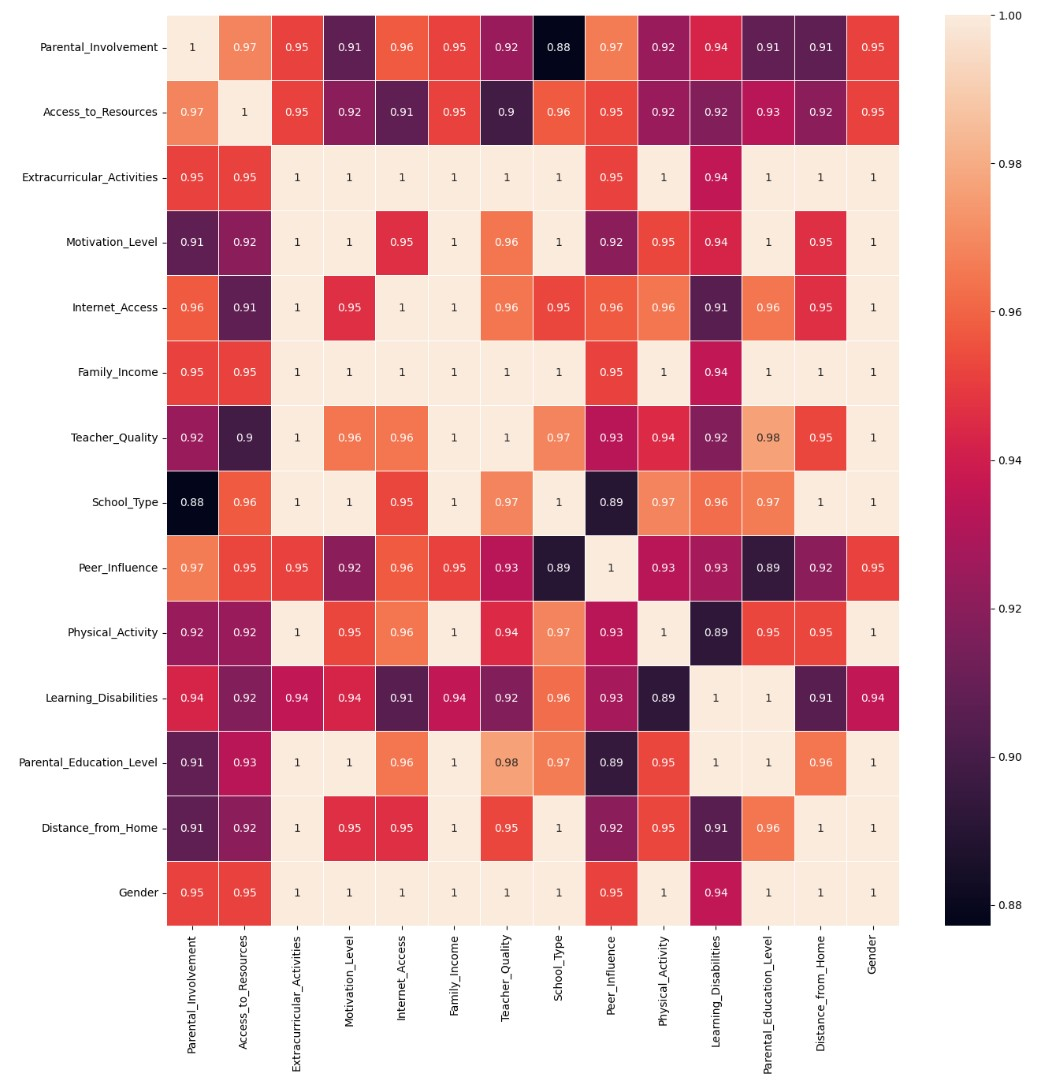
\includegraphics[width=1\textwidth]{./images/icon4.jpg}
    
\end{center}
Ο πίνακας Cramer's V χρησιμοποιείται για να μετρήσει τη συσχέτιση μεταξύ κατηγορικών μεταβλητών.

\begin{center}
    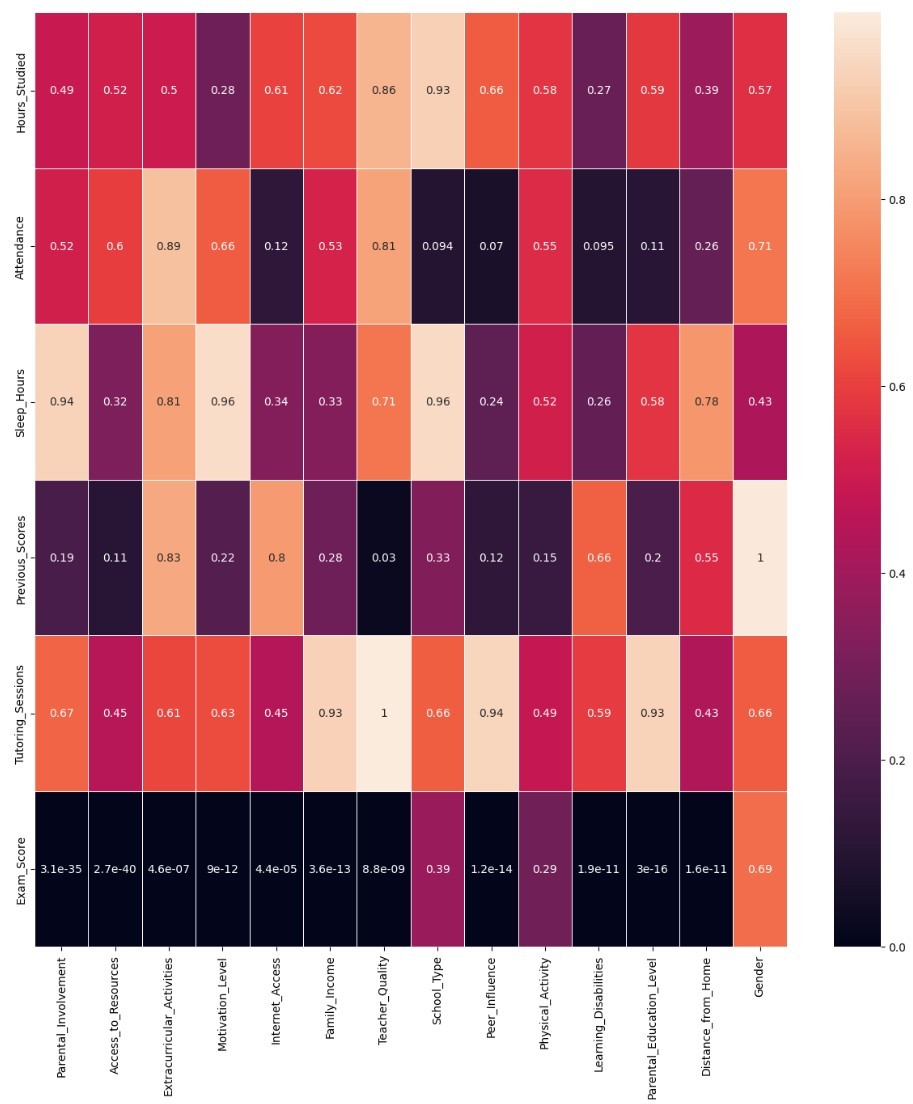
\includegraphics[width=1\textwidth]{./images/icon5.jpg}
    
\end{center}

\begin{center}
    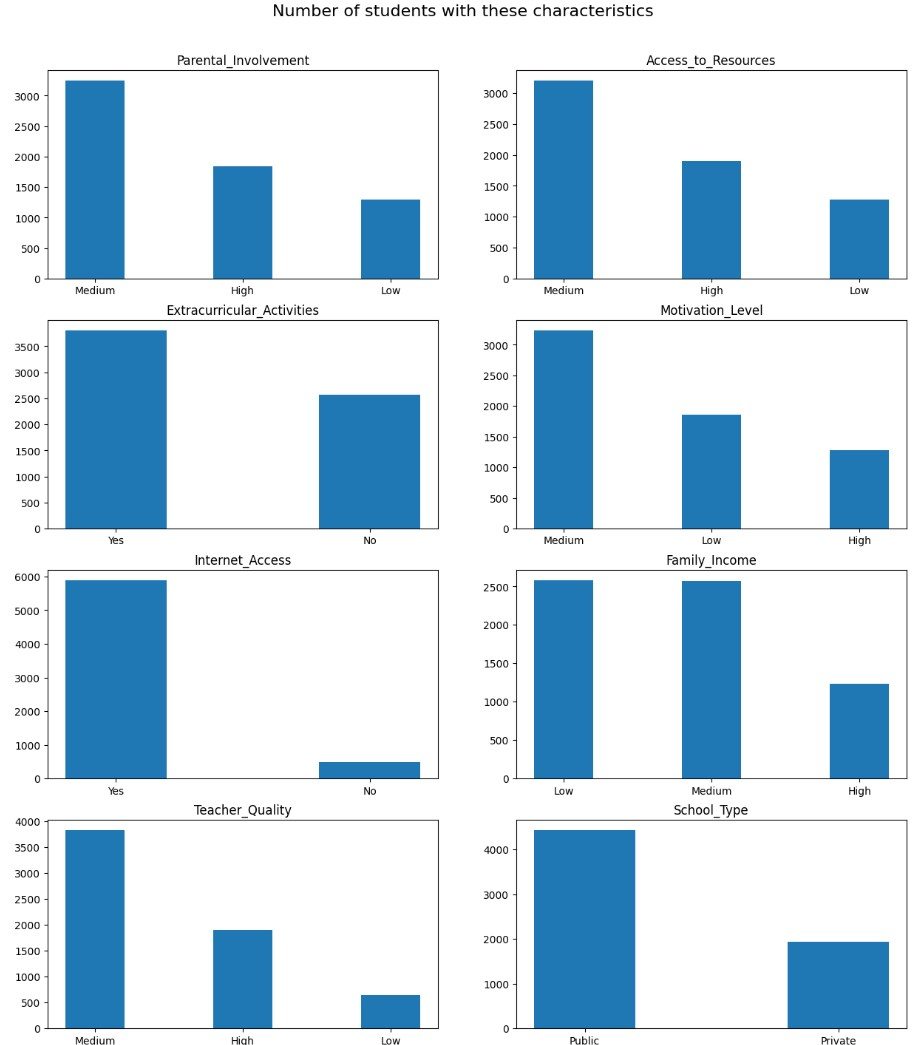
\includegraphics[width=0.9\textwidth]{./images/icon6.jpg}
    
\end{center}
\begin{center}
    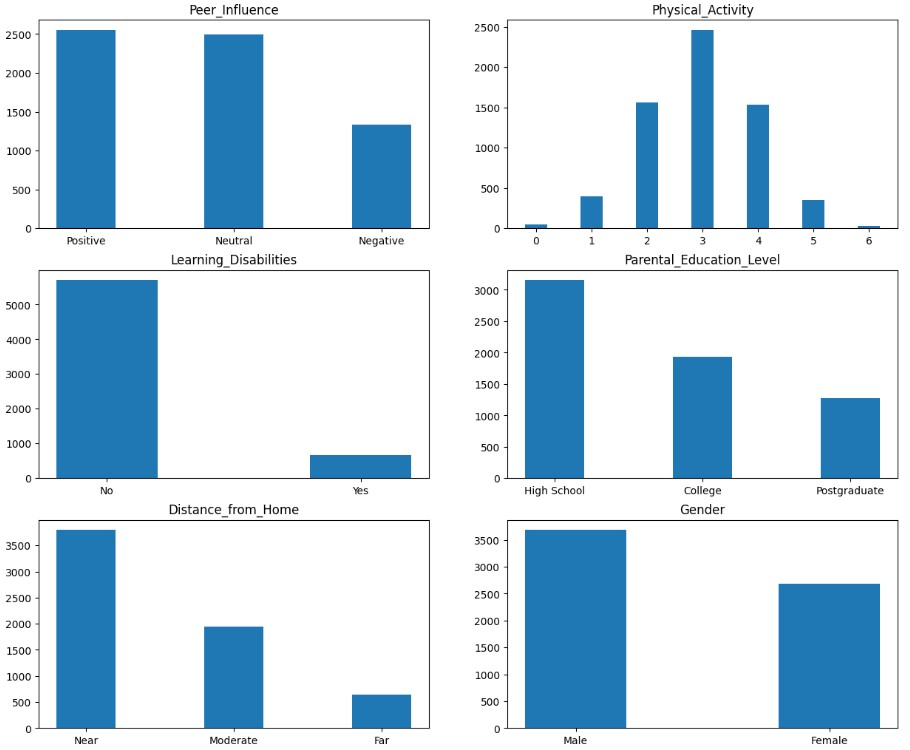
\includegraphics[width=0.9\textwidth]{./images/icon7.jpg}
    
\end{center}
\subsection{Επιλογή χαρακτηριστικών}

Η επιλογή των χαρακτηριστικών που θα χρησιμοποιήσουμε για την πρόβλεψη του στόχου αποτελέι σημαντικό βήμα. Απο την μια προσπαθούμε να επιλέξουμε όλα τα σημαντικά χαρακτηριστικά έτσι ώστε να αποφύγουμε την υποπροσαρμογή, δηλαδή το μοντέλο μας να μην έχει τις απαραίτητες πληροφορίες για να αποτυπώσει την σχέση μεταξύ των δεδομένων και της μεταβλητής στόχου και απο την άλλη προσπαθούμε να επιλέξουμε όσο το δυνατό λιγότερα μη σημαντικά χαρακτηριστικά έτσι ώστε να αποφύγουμε την υπερπροσαρμογή, δηλαδή το μοντέλο μας να αποδίδει πολύ καλά στα δεδομένα εκπαίδευσης αλλά να αδυνατεί να γενικεύσει σε νέα δεδομένα.Αρχικά θα ορίσουμε 8 στο σύνολο μοντέλα παλινδρόμισης για τα οποία θα εξετάσουμε την απόδοση τους μέσω μιας μετρικής για κάθε συνδυασμό χαρακτηριστικών. Τα μοντέλα παλινδρόμισης τα οποία θα εξετάσουμε είναι τα εξής:\\
\begin{enumerate}
    \item Πολυωνιμικό μοντέλο παλινδρόμισης
    \item Γραμμική παλινδρόμιση
    \item Decision Tree παλινδρόμιση
    \item Random Forest παλινδρόμιση
    \item Support Vector παλινδρόμιση
    \item Gradient Boosting παλινδρόμιση
    \item Παλινδρόμιση Ridge
    \item Παλινδρόμιση Lasso\\
\end{enumerate}

 Για την πραγματοποίηση της παραπάνω διαδικασίας θα χρησιμοποιήσουμε τον αλγόριθμο Sequential feature selection (SFS). Θα μπορούσαμε να κάνουμε την διαδικασία αυτή και μέσω των πινάκων συσχέτισης Pearson, Cramer's V και ANOVA διαγράφοντας για κάθε ζεύγος μεταβλητών με ισχυρή συσχέτιση την μια απο τις δύο μεταβλητές αλλά με την διαφορά πως δεν θα είχαμε τόσο καλά αποτελέσματα όσο με την μέθοδο SFS. Η μέθοδος SFS με επιλογή για backwards selection ξεκινά με το πλήρες σύνολο χαρακτηριστικών. Το σύνολο εκπαίδευσης χωρίζεται σε k=cross-validation ίσα μέρη(folds). Σε κάθε επανάληψη, αφαιρείται ένα χαρακτηριστικό από το τρέχον σύνολο, και το μοντέλο εκπαιδεύεται χρησιμοποιώντας τα εναπομείναντα χαρακτηριστικά. Το μοντέλο εκπαιδεύεται k φορές, χρησιμοποιώντας κάθε φορά ένα διαφορετικό fold ως σύνολο δοκιμής (test set), ενώ τα υπόλοιπα k-1 folds χρησιμοποιούνται ως σύνολο εκπαίδευσης(training set). Η απόδοση για κάθε αφαίρεση χαρακτηριστικού αξιολογείται με βάση τον μέσο όρο της απόδοσης για κάθε επιλογή fold ώς test set χρησιμοποιώντας κάποιο προκαθορισμένο κριτήριο, όπως το μέσο τετραγωνικό σφάλμα (MSE). Το χαρακτηριστικό που οδηγεί στη μικρότερη μείωση της απόδοσης αφαιρείται οριστικά από το σύνολο. Η διαδικασία συνεχίζεται μέχρι να επιτευχθεί ο επιθυμητός αριθμός χαρακτηριστικών. Για κάθε ένα απο τα μοντέλα παλινδρόμισης που αναφέραμε παραπάνω εντοπίσαμε τα χαρακτηριστικά τα οποία οδηγούν στο μικρότερο μέσο τετραγωνικό σφάλμα. Για την καλύτερη κατανόηση της μεθόδου, παρουσιάζεται παρακάτω η γραφική παράσταση του βέλτιστου αρνητικού μέσου τετραγωνικού σφάλματος. Η γραφική αφορά το μοντέλο παλινδρόμησης Decision Tree και βασίζεται στα χαρακτηριστικά που ελαχιστοποιούν το μέσο τετραγωνικό σφάλμα. Συγκεκριμένα, η γραφική απεικονίζει τη σχέση μεταξύ του αριθμού των χαρακτηριστικών και του μέσου τετραγωνικού σφάλματος, όπως αυτά επιλέχθηκαν μέσω της συγκεκριμένης μεθόδου.

\begin{center}
    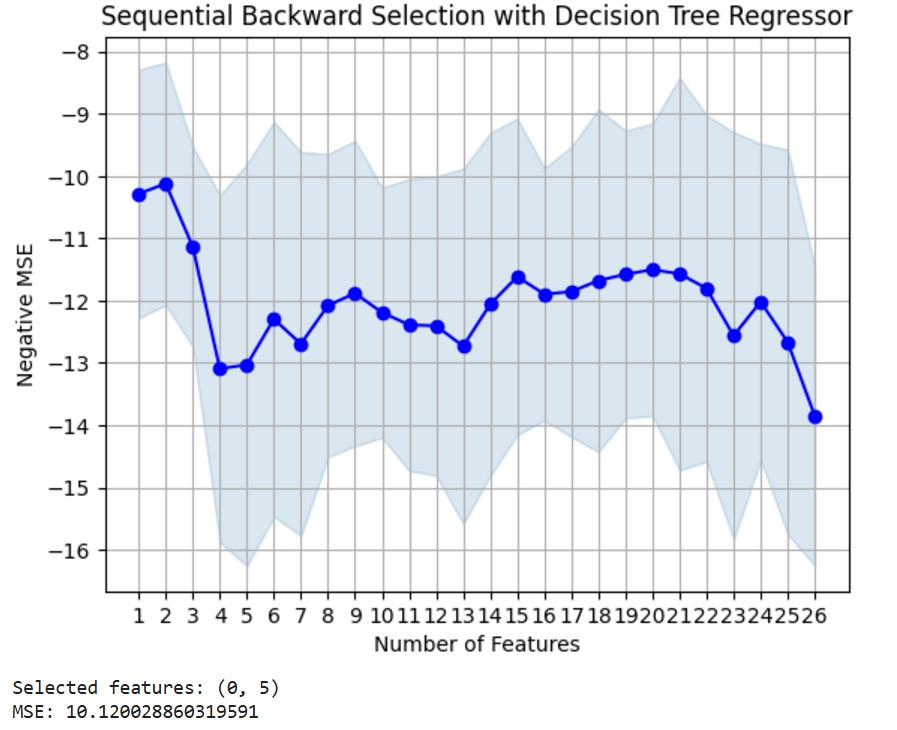
\includegraphics[width=0.9\textwidth]{./images/icon8.jpg}
    
\end{center}

Μπορούμε εύκολα να παρατηρήσουμε πως το το μεγαλύτερο αρνητικό μέσο τετραγωνικό σφάλμα επιτυγχάνετε για αριθμό χαρακτηριστικών ίσο με 2. Το αντίστοιχο καλύτερο μέσο τετραγωνικό σφάλμα είναι ίσο με 10.12 και επιτυγχάνετε χρησιμοποιώντας την πρώτη και έκτη στήλη του πίνακα δεδομένων.

\subsection{Επιλογή υπερπαραμέτρων}
Για κάθε ένα από τα μοντέλα παλινδρόμησης που ορίσαμε παραπάνω, πραγματοποιήσαμε βελτιστοποίηση υπερπαραμέτρων (hyperparameter tuning) χρησιμοποιώντας τη μέθοδο GridSearchCV. Η βελτιστοποίηση έγινε για τα αντίστοιχα χαρακτηριστικά που επιλέχθηκαν ως βέλτιστα μέσω της μεθόδου Sequential Forward Selection (SFS). Στη διαδικασία, θέσαμε cross-validation = 10 και επιλέξαμε ως μετρική απόδοσης το μέσο τετραγωνικό σφάλμα(MSE). Η διαδικασία βελτιστοποίησης πραγματοποιήθηκε σε δύο στάδια. Aρχικά, εξετάσαμε ένα εύρος παραμέτρων γύρω από τις προεπιλεγμένες τιμές (default parameters), ώστε να αποκτήσουμε μια αρχική εικόνα για τη συμπεριφορά του μοντέλου. Στη συνέχεια, εστιάσαμε στις παραμέτρους που ανέδειξε η πρώτη διαδικασία ως πιο σημαντικές, προσαρμόζοντας το εύρος των τιμών τους για πιο λεπτομερή αναζήτηση. Με αυτόν τον τρόπο καταφέραμε να βελτιώσουμε περαιτέρω την απόδοση των μοντέλων μας, εξασφαλίζοντας καλύτερα αποτελέσματα.

Η μέθοδος GridSearchCV λειτουργεί ώς ακολούθως.
Το σύνολο εκπαίδευσης χωρίζεται σε k=cross-validation ίσα μέρη(folds). Στη συνέχεια, για κάθε συνδυασμό υπερπαραμέτρων που ορίζει ο χρήστης το μοντέλο εκπαιδεύεται k φορές, χρησιμοποιώντας κάθε φορά ένα διαφορετικό fold ως σύνολο δοκιμής (test set), ενώ τα υπόλοιπα k-1 folds χρησιμοποιούνται ως σύνολο εκπαίδευσης(training set). Η απόδοση κάθε συνδυασμού υπερπαραμέτρων αξιολογείται με βάση τον μέσο όρο της απόδοσης για κάθε επιλογή fold ώς test set. Τέλος, επιλέγεται ο συνδυασμός υπερπαραμέτρων που βελτιστοποιεί τη μετρική απόδοσης.
\subsection{Επιλογή μοντέλου}
Για να βρούμε το τελικό βέλτιστο μοντέλο παλινδρόμισης απο αυτά που εξετάσαμε κατασκευάσαμε το ραυδόγραμμα του μέσου τετραγωνικού σφάλματος για κάθε ένα απο τα μοντέλα παλινδρόμισης που αναλύσαμε. Το ραυδόγραμμα αυτό παρουσιάζεται παρακάτω: 

\begin{center}
    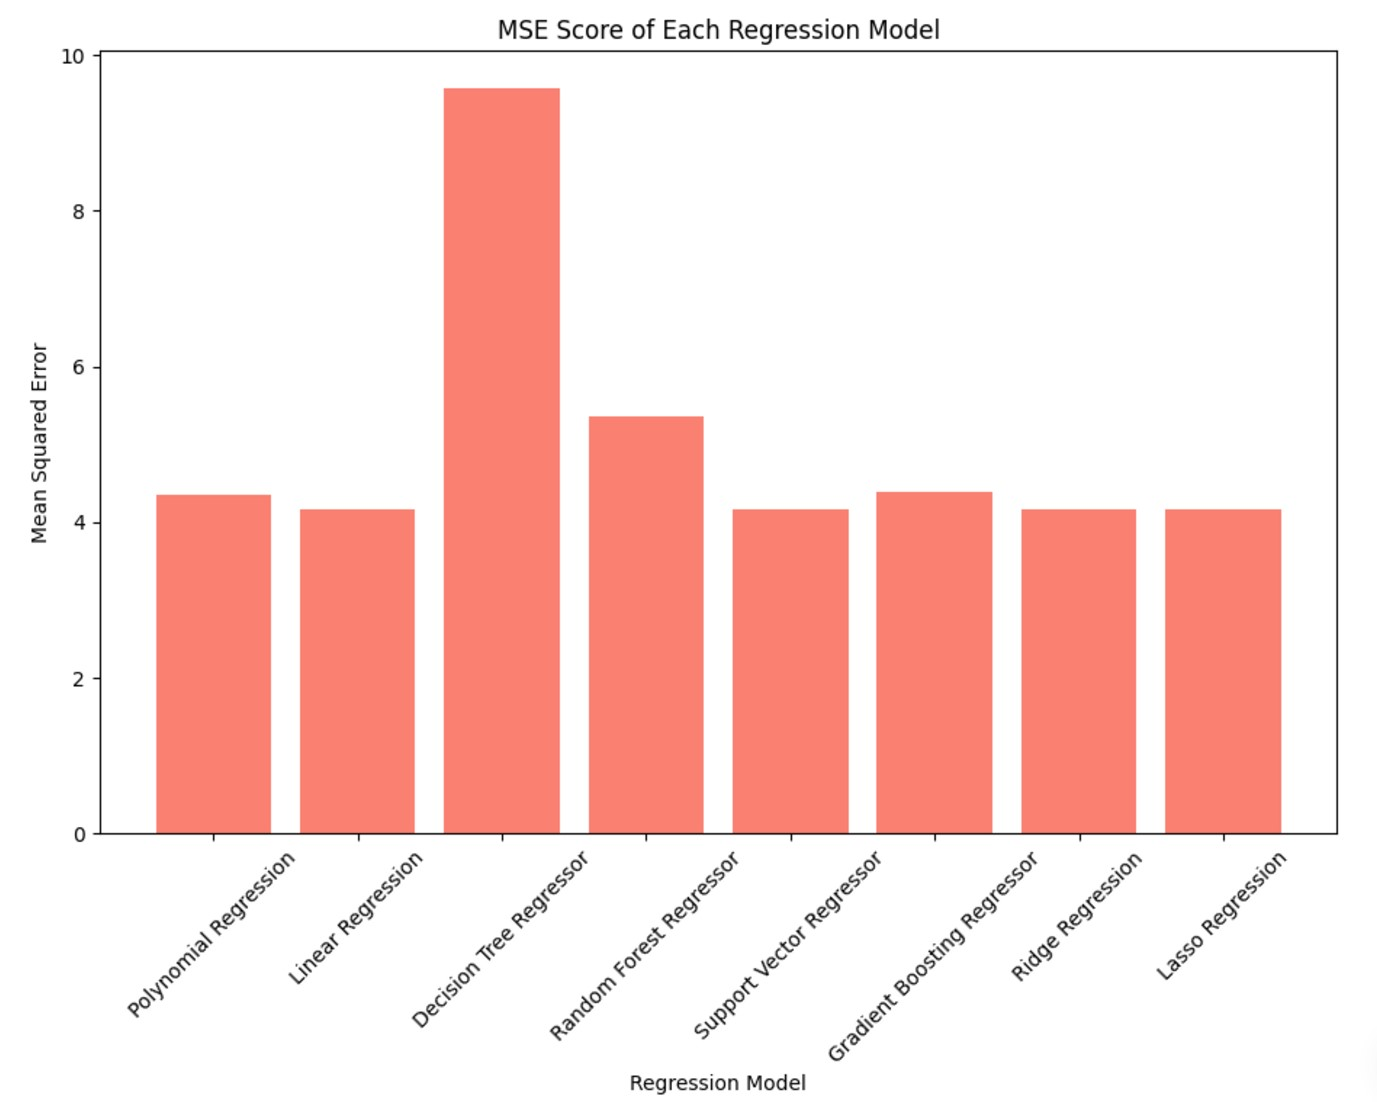
\includegraphics[width=0.9\textwidth]{./images/icon9.jpg}
    
\end{center}

Το μοντέλο το οποίο περιγράφει καλύτερα τα δεδομένα μας και προβλέπει σε καλύτερο βαθμό τον βαθμό του μαθητή με βάση την μετρική απόδοσης MSE είναι το μοντέλο παλινδρόμισης Lasso με μέσο τετραγωνικό σφάλμα ίσο με 4.155, επομένως έχουμε RMSE=\(\sqrt{MSE}=2.038\) και αυτό σημαίνει πως κατά μέσο όρο η πρόβλεψη μας για κάθε βαθμό εξέτασης διαφέρει κατά 2.038 μονάδες απο την πραγματική τιμή. Με βάση την ανάλυση που κάναμε για τις υπερπαραμέτρους το μοντέλο αυτό έχει παραμέτρους ίσες με ρυθμό κανονικοποίησης(alpha) ίσο με 0.0001, μέγιστο αριθμό επαναλήψεων(max\_iter) ίσο με 500 και ανοχή σύγκλισης(tol) ίση με 0.1.Για να εξετάσουμε περαιτέρω την απόδοση του μοντέλου μας υπολογίσαμε τον συντελεστή προσδιορισμού \( R^2 \), ο οποίος ισούται με 0.733  επομένως το μοντέλο μας εξηγά το 73.3\(\%\) της μεταβλητότητας του Exam Score. Τέλος, κατασκευάσαμε το γράφημα που φαίνετε παρακάτω όπου παρουσιάζει τις προβλεπόμενες τιμές του test set σε σχέση με τις αντίστοιχες πραγματικές τιμές. 


\begin{center}
    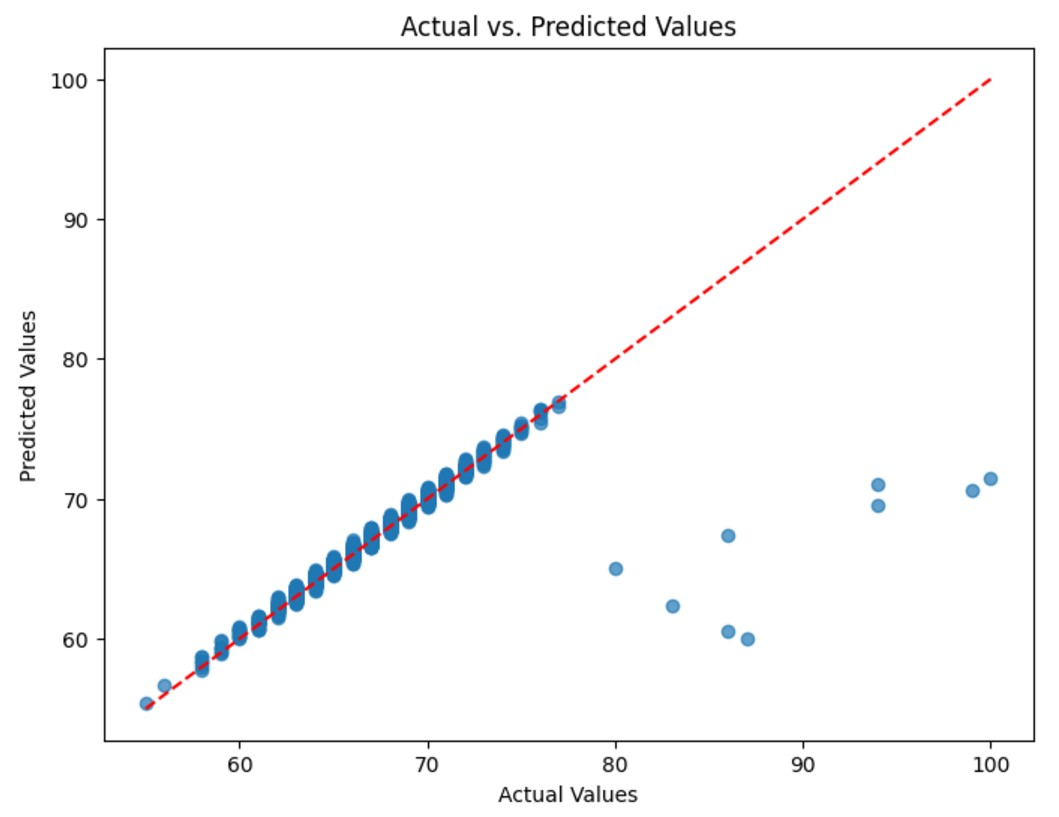
\includegraphics[width=0.9\textwidth]{./images/icon10.jpg}
    
\end{center}

Μπορούμε να παρατηρήσουμε πως το μοντέλο μας με βάση την γραφική υπολογίζει σε πολύ ικανοποιητικό βαθμό τον βαθμό του μαθητή για τιμές μικρότερες του 80. Για τιμές μεγαλύτερες απο 80 δεν μπορούμε να πούμε το ίδιο. Αυτό μπορεί να οφείλετε στο ότι δεν υπάρχουν αρκετοί μαθητές οι οποίοι πήραν βαθμό μεγαλύτερο απο 80 στο training set, επομένως το μοντέλο μηχανικής μάθησης που δημιουργήσαμε δεν έχει αρκετά δεδομένα για να προβλέψει ικανοποιητικά τον τελικό βαθμό του μαθητή. Επίσης λόγω της μεγάλης διαφοράς στο πλήθος των δεδομένων στο training set για βαθμούς μικρότερους απο 80 σε σχέση με μεγαλύτερους απο αυτό, μπορεί να οδήγησε το μοντέλο μας σε υπερβολική εστίαση στα δεδομένα μικρότερα απο 80(biased ώς πρός αυτά τα δεδομένα) αφού τελικά θα οδηγούσε σε μικρότερο ολικό μέσο τετραγωνικό σφάλμα σε αντίθεση με το να το έκανε γενίκευση(generalize) και για τιμές μεγαλύτερες απο 80.

\newpage
\section{Το μοντέλο παλινδρόμισης Lasso}
\subsection{Έγκριση ειδικού πλαισίου χωροταξικού σχεδιασμού}
Αναλύεται η διαδικασία έγκρισης του πλαισίου.

\subsection{Καθορισμός περιοχών αιολικής προτεραιότητας}
Αναλύονται οι παράγοντες επιλογής περιοχών.

\subsection{Παράμετροι που καθορίζουν τις αποστάσεις}
Παρουσιάζονται τα κριτήρια για τις αποστάσεις υποδομών.

\newpage
\section{Σύγκριση με έρευνες}
hb
\newpage
\section{Βιβλιογραφία}

\end{document}